\chapter{Amplifier Classes}
The generic power amplifier consists of a transistor with a DC bias and AC coupled to the RF input and output ports. For the sake of simplicity this work will only describe the operation of field effect transistor amplifiers. The major source of power consumption of an amplifier comes from the drain source current and voltage that occurs during operation. Power amplifiers come in a variety of classes, and the most commonly used ones are A, B, AB, C, D, E, and F. Classes A through C can be described by the conduction angle of the device and modeling the transistor as a current source. The conduction angle is the amount of current flowing through the transistor from drain to source during a single cycle of the AC signal being amplified and ranges from 0 to $2\pi$ \cite{Colantonio1998}. Classes D through F are defined as switching amplifiers and vary due to the matching networks which shape the waveforms of the current and voltage at the drain and gate of the device \cite{Sokal1975}. This chapter will describe a high level overview of the various amplifier classes and discuss the limitations of each in practice.

%For class A, the conduction angle is $2\pi$ meaning current is always flowing when the amplifier is on increasing the power consumption. Class A does have the advantage of having the highest gain at a given frequency compared to other classes and also can operate near the frequency limit of a transistor .\cite{} Class A also has the highest linearity, lowest harmonic distortion, and is advantageous when high dynamic range is required .\cite{C.Cripps2006} Class B has a conduction angle of $\pi$ so current only flows during half the cycle of the AC signal reducing power consumption. Class AB has a conduction angle between $\pi$ and $2\pi$. Class E is a type of harmonic termination that uses capacitive terminations at the output to achieve 100\% efficiency.

% Citations are wrong above!

\section{Efficiency of Amplifiers}

To reduce the power consumption of a power amplifiers, two major concepts are important: zero voltage switching (ZVS) and zero voltage derivative switching (ZVDS). ZVS is when there is zero voltage when the amplifier is switched on and conducting so while current flows through the output no power is consumed. ZVDS is when there is no overlap between the voltage and current waveforms so no power is consumed during the switching. An amplifier can be 100\% if it achieves ZVS and ZVDS because no power would be consumed at any point in the amplification process. A measure of amplifier efficiency is the power added efficiency (PAE) defined in Equation \ref{pae}. PAE is a measure of how efficient an amplifier is able to convert the input DC power into RF power gain. Ideally all of the DC power used to power the amplifier would be used to increase the input RF power. The maximum limit for a lossless system is 100\%, for example if a power amplifier consumed 1 Watt and was able to output 1.001 Watt of RF power from 1 mW of RF input power, the PAE would be 100.\% because all of the DC power was used to increase the RF power.

\begin{equation}\label{pae}
  PAE,\% = \frac{RF\;Power_{out} - RF\\Power_{in}}{DC\;Power}
\end{equation}

Another measure of amplifier efficiency is the drain efficiency which is the proportion of the output power of the fundamental harmonic over the DC power consumed seen in Equation \ref{drain_eff}. The drain efficiency is typically used when talking about the theory behind the different amplifier classes. In practice, PAE is used as the metric to compare power amplifier efficiency because it takes in account RF input power which is relatively large compared to small signal amplifiers. Small signal amplifiers operate at a bias point that can be assumed to be linear for small input powers. Power amplifiers are large signal devices that operate in the non-linear regions of transistor.

\begin{equation}\label{drain_eff}
  \eta, \% = \frac{P_{Fundamental}}{DC\;Power}
\end{equation}

\section{Current Source Amplifiers}

\subsection{Class A Amplifier}

\begin{figure}
  \centering
  % Requires \usepackage{graphicx}
  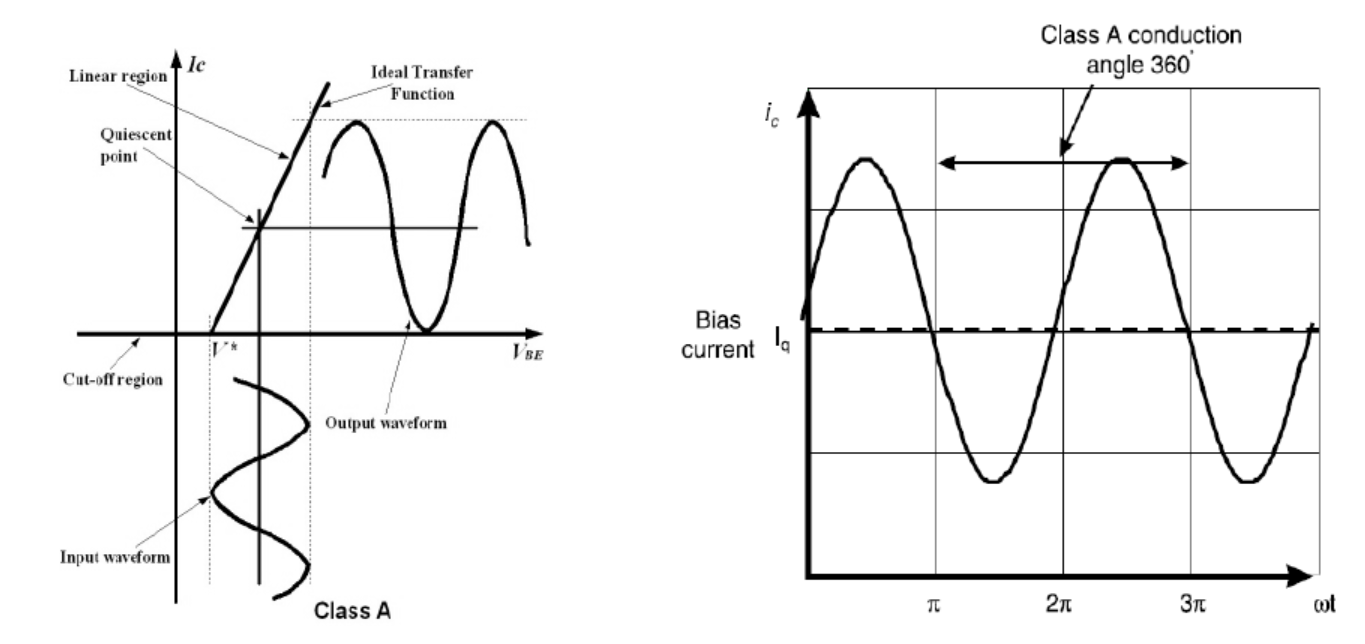
\includegraphics[width=6in]{figures/classes/classa}
  \caption{Class A Bias Point and Conduction Cycle \cite{Rosu2001}}\label{classa_bias}
\end{figure}

The class A amplifier uses a bias that results in a conduction angle of $2\pi$, seen in Figure \ref{classa_bias}, and a theoretical quiescent current of 50\% the maximum drain current. This results in power always being consumed due to the constant bias current and voltage present at the drain of the amplifier. The bias point is chosen so the transistor operates in the active region which can be seen in Figure \ref{classa_bias}. The constant power consumption limits the maximum efficiency of the class A amplifier for a continuous wave (CW) signal to 50\% \cite{C.Cripps2006}.

%The class A amplifier is similar to the small signal amplifier in many ways

The class A amplifier is the most linear of all classes due to the conduction angle that provides ideally no clipping of the current or voltage waveforms. The high linearity allows the class A amplifier to have the lowest intermodulation distortion (IMD) of all the amplifier classes. The downside of the linearity is that the input drive level is proportional to the IMD present at the output of the amplifier. Class A amplifiers are also able to operate closer to the highest operating frequency of a transistor because it does't use the harmonics present in the amplifier for it's amplification \cite{Rosu2001}. %ham paper

%Fix all the citations lol


\subsection{Class B Amplifier}

\begin{figure}
  \centering
  % Requires \usepackage{graphicx}
  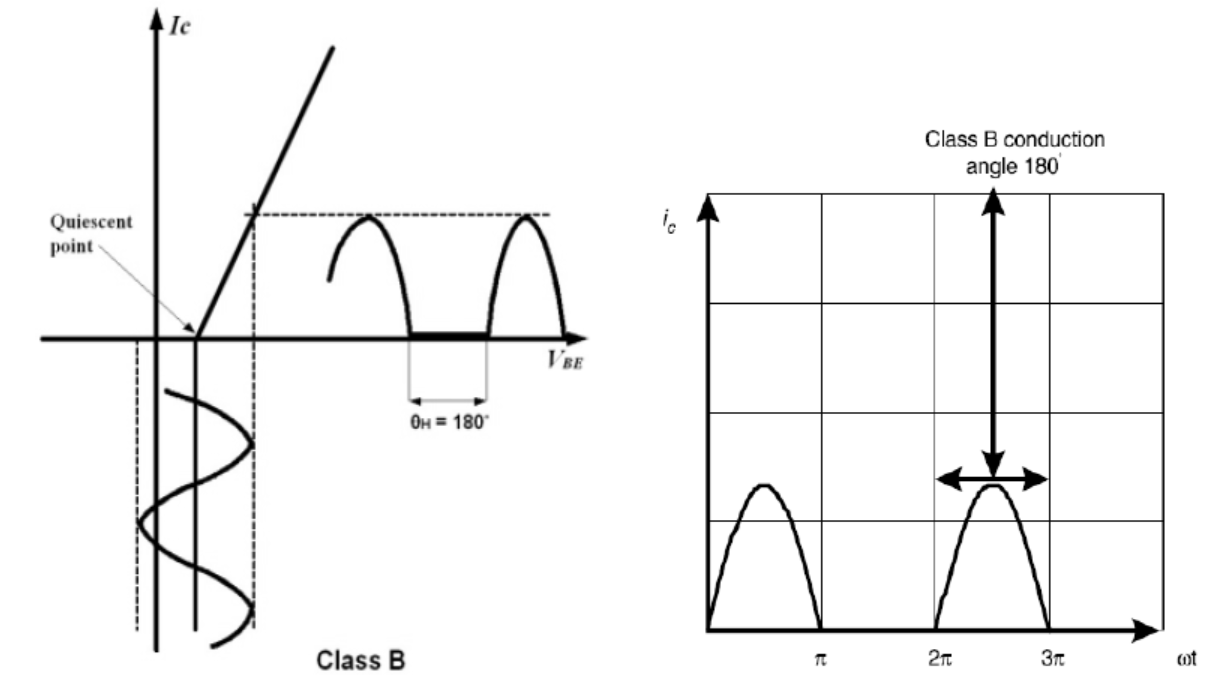
\includegraphics[width=6in]{figures/classes/classb_bias}\\
  \caption{Class B Bias Point and Conduction Cycle \cite{Rosu2001}}\label{classb_bias}
\end{figure}

Class B uses a conduction angle of $\pi$ resulting in a half sinusoid waveform for the drain current seen in Figure \ref{classb_bias} with a theoretical quiescent current of 0 A. The maximum efficiency for a CW signal is 78.5\%. The reduced conduction angle causes the required input power to achieve the maximum efficiency to be 6 dB higher compared to the class A amplifier \cite{C.Cripps2006}.
The drain current is proportional to the input signal so the Class B amplifier is considered a linear amplifier but will result in harmonic distortion due to the clipping of the drain current. The output is usually filtered to reduce the harmonic distortion\cite{Raab2003}.
In most applications, the class B amplifier is used in a push pull configuration to reduce distortion by providing a full sine wave output and maintain greater efficiency than a class A amplifier. Also instead of setting the quiescent current to 0, the drain current is typically set to 10\% of the max drain current of the transistor to reduce the harmonic distortion. An interesting result of the push pull configuration is that even harmonics subtract one another out while odd harmonics add together \cite{Rosu2001}.


\subsection{Class AB Amplifier}

\begin{figure}
  \centering
  % Requires \usepackage{graphicx}
  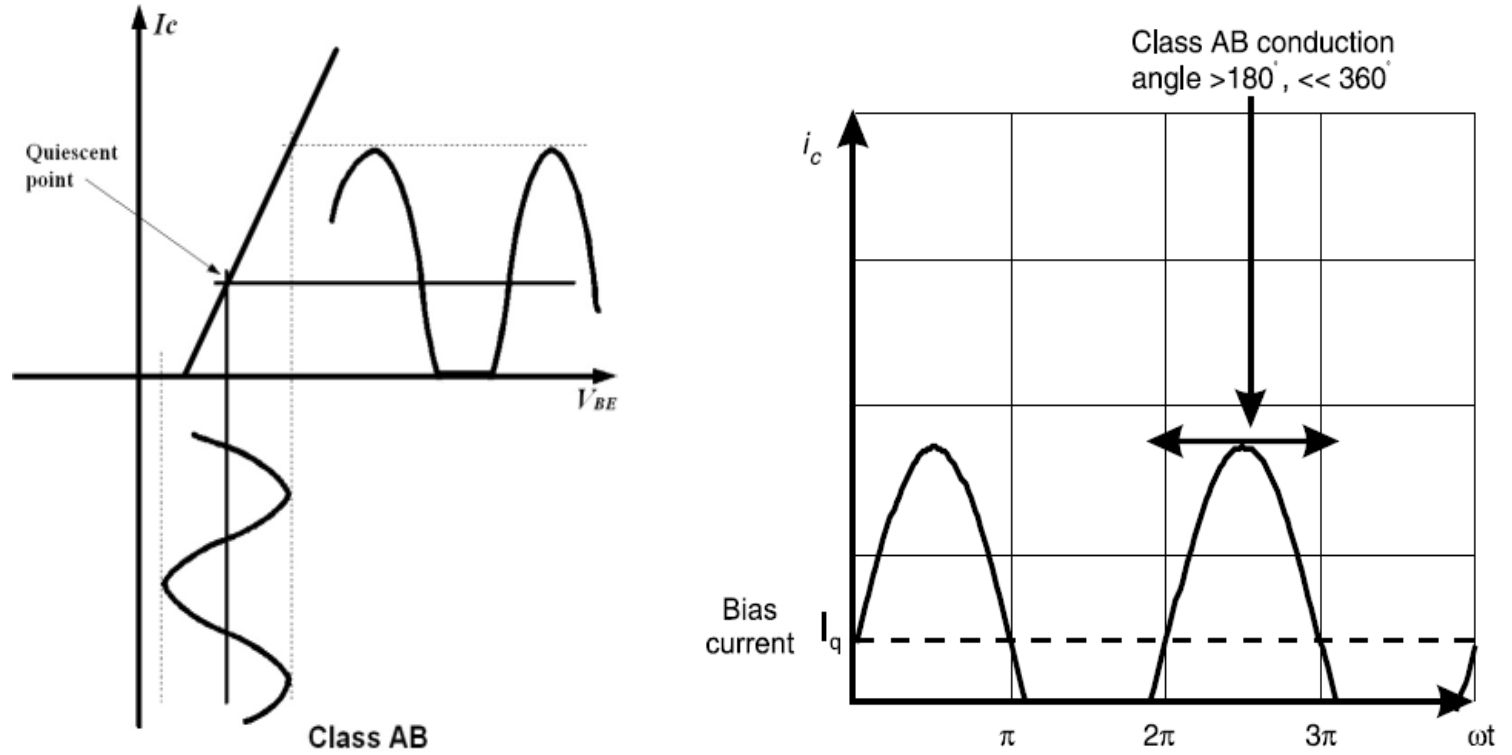
\includegraphics[width=6in]{figures/classes/classab_bias}\\
  \caption{Class AB Bias Point and Conduction Cycle \cite{Rosu2001}}\label{classab_bias}
\end{figure}

The class AB amplifier uses a conduction angle ranging between $\pi$ and $2\pi$ and is a compromise between class A and class B amplifiers. The drain efficiency lies between 50\% and 78.5\% with approximately the same output power as the class A amplifier \cite{C.Cripps2006}. The bias point and conduction cycle can be seen in Figure \ref{classab_bias}. The class AB amplifier offers a wider dynamic range than class A or class B because the conduction angle is proportional to the drain current which also results in the class AB amplifier being a non-linear amplifier \cite{C.Cripps2006}.

\subsection{Class C Amplifier}

\begin{figure}
  \centering
  % Requires \usepackage{graphicx}
  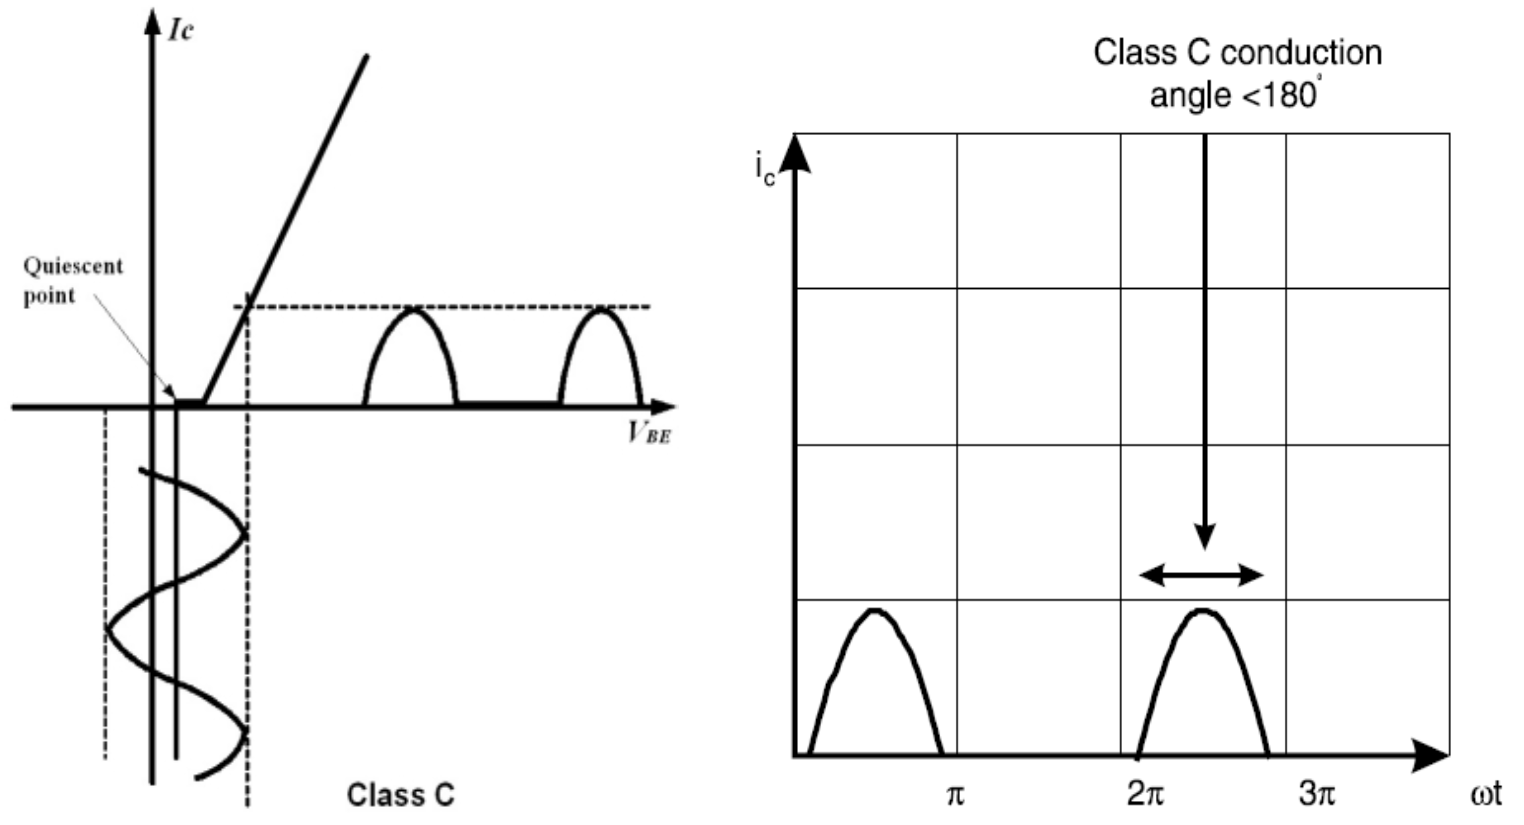
\includegraphics[width=6in]{figures/classes/classc_bias}\\
  \caption{Class C Bias Point and Conduction Cycle \cite{Rosu2001}}\label{classc_bias}
\end{figure}

The class C amplifiers is biased such that the quiescent current is 0 A and the conduction angle is between $0$ and $\pi$ seen in Figure \ref{classc_bias}. The class C amplifier is non-linear with a higher efficiency than class B with a maximum drain efficiency of 100\% at zero conduction angle but will have zero gain. In practice, the class C amplifier has a conduction angle slightly less than $\pi$ for a maximum efficiency of 85\% while still having a useful gain \cite{Raab2003}. The class C has the highest harmonic distortion of all the current source amplifier classes which will be shown in the following section. The harmonic distortion requires significant filtering at the output of the amplifier. Class C amplifiers aren't typically used for microwave power amplifiers due to the large negative voltage present at the gate of the transistor which can cause reverse breakdown in the transistor \cite{C.Cripps2006}. The class C amplifier offers a tradeoff of higher efficiency but with higher harmonic distortion and lower output power level compared to the other current source amplifier classes.

\subsection{Harmonic Distortion}

The current source power amplifiers can be generalized to a power amplifier with various conduction angles and the drain efficiencies. The  output power and harmonic distortion can be described as a function of conduction angle seen in Equations \ref{eq:cond_eff}, \ref{eq:cond_pout}, and \ref{eq:cond_current} \cite{Hella}. Table \ref{table:waveform_param} defines the various parameters to the various equations. Figure \ref{fig:bias_current_harmonic} shows the normalized output current harmonics versus conduction angle. At a conduction angle of $2\pi$, the output has minimal harmonic distortion with only the fundamental and DC component  present. The DC component is easily removed by coupling capacitor. As conduction angle increase, the other harmonic amplitudes increase which causes increased harmonic distortion and the DC power is reduced increasing the efficiency. At zero conduction angle, the transistor won't conduct any current and all of the harmonic amplitudes drop to 0. Figure \ref{fig:bias_power_eff} shows the RF power relative to class A and efficiency versus conduction angle assuming the harmonics are removed and the transistor is optimally loaded. A power amplifier is said to be properly loaded if the load resistance is equal to the DC drain voltage minus the knee voltage of the transistor divided by the fundamental drain current, see Equation \ref{eq:opt_load} \cite{Hella}.

The generalized form of the current source amplifiers are not able to ever achieve ZVS due to the constant drain voltage waveform present at the output which is required to bias the amplifier. And current source amplifiers can only achieve ZVDS at a conduction angle of 0 radians which results in 0 power delivered to the load. To achieve 100\% efficiency and have a practical gain we look to the switching amplifier.
%In the equations, $v_{dd}$ is the drain voltage, $v_{sat}$ is the saturation voltage of the transistor, $\theta$ is the conduction angle in radians,

\begin{table}
    \caption{Table of Current Source Waveform Parameters}
    \label{table:waveform_param}
        \begin{center}
            \begin{tabular}{|l|l|l|}
              \hline
              % after \\: \hline or \cline{col1-col2} \cline{col3-col4} ...
              Parameter & Definition & Units\\ \hline
              $I_m$ & Maximum drain current of transistor & A \\ \hline
              $I_n$ & Magnitude of current harmonic $n$ & A \\ \hline
              $v_{dd}$ & DC drain voltage & V\\ \hline
              $v_{knee}$ & Knee voltage of transistor & V\\ \hline
              $v_{sat}$ & Saturation voltage of transistor & V \\ \hline
              $\theta$ & Conduction angle & Radians\\ \hline

            \end{tabular}
        \end{center}
\end{table}

\begin{equation}\label{eq:cond_eff}
  \eta_{Drain}, \% = \frac{v_{dd} - v_{sat}}{v_{dd}} \frac{\theta - sin\theta}{4(sin\frac{\theta}{2} - \frac{\theta}{2} cos\frac{\theta}{2}) }
\end{equation}

\begin{equation}\label{eq:cond_pout}
  P_{out} = \frac{1}{2}(v_{dd} - v_{sat} )\frac{I_m}{2\pi}(\theta - sin\theta)
\end{equation}

\begin{equation}\label{eq:cond_current}
  I_n = \frac{1}{\pi}\int_{-\frac{\theta}{2}}^{\frac{\theta}{2}} \frac{I_m}{1 - cos(\frac{\theta}{2})} (cos\alpha - cos(\frac{\theta}{2}))cos(n\alpha) \; d\alpha
\end{equation}

\begin{equation}\label{eq:opt_load}
  R_{opt} = \frac{v_{dd}-v_{knee}}{I_{Fundemetnal}}
\end{equation}

\begin{figure}
  \centering
  % Requires \usepackage{graphicx}
  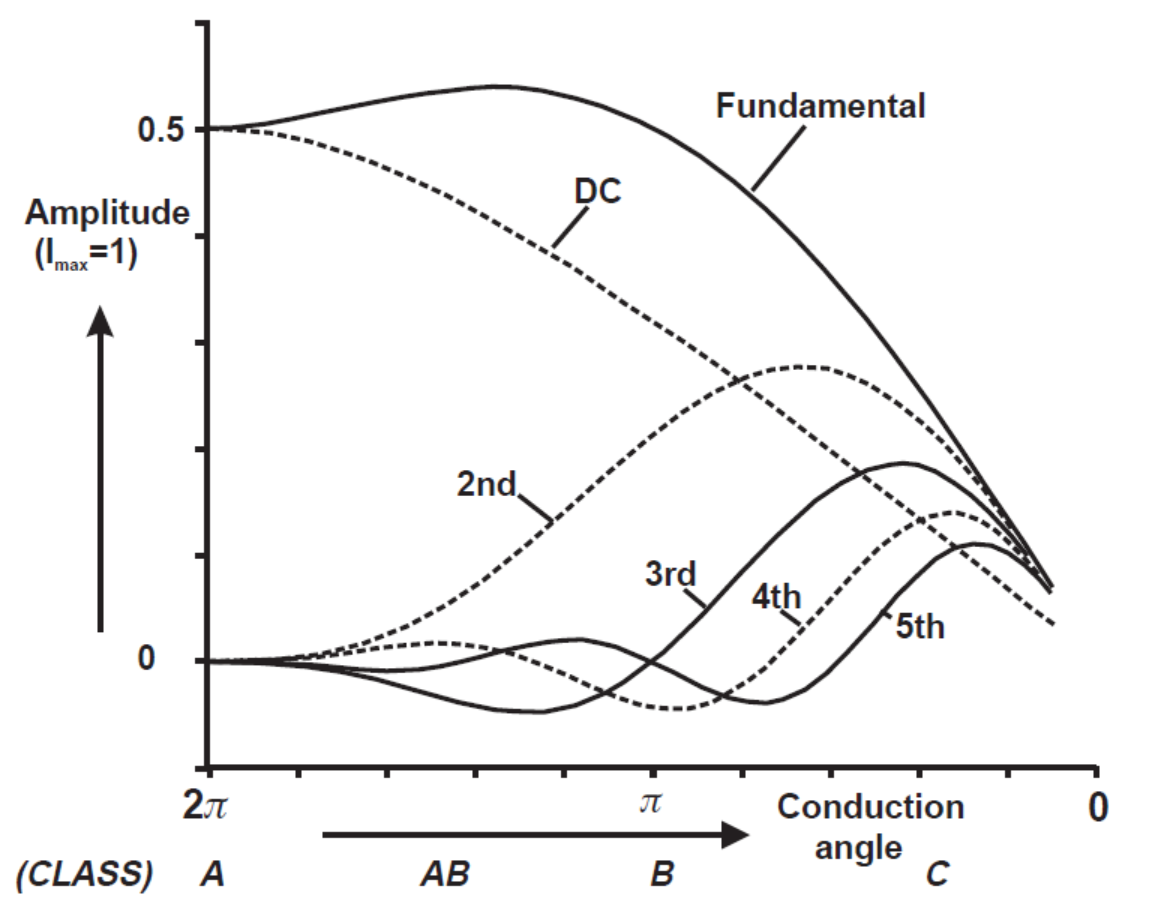
\includegraphics[width=4in,height=4in,keepaspectratio]{figures/classes/bias_current_harmonic}\\
  \caption{Normalized Current Harmonic Amplitude versus Conduction Angle \cite{C.Cripps2006}}
  \label{fig:bias_current_harmonic}
\end{figure}

\begin{figure}
  \centering
  % Requires \usepackage{graphicx}
  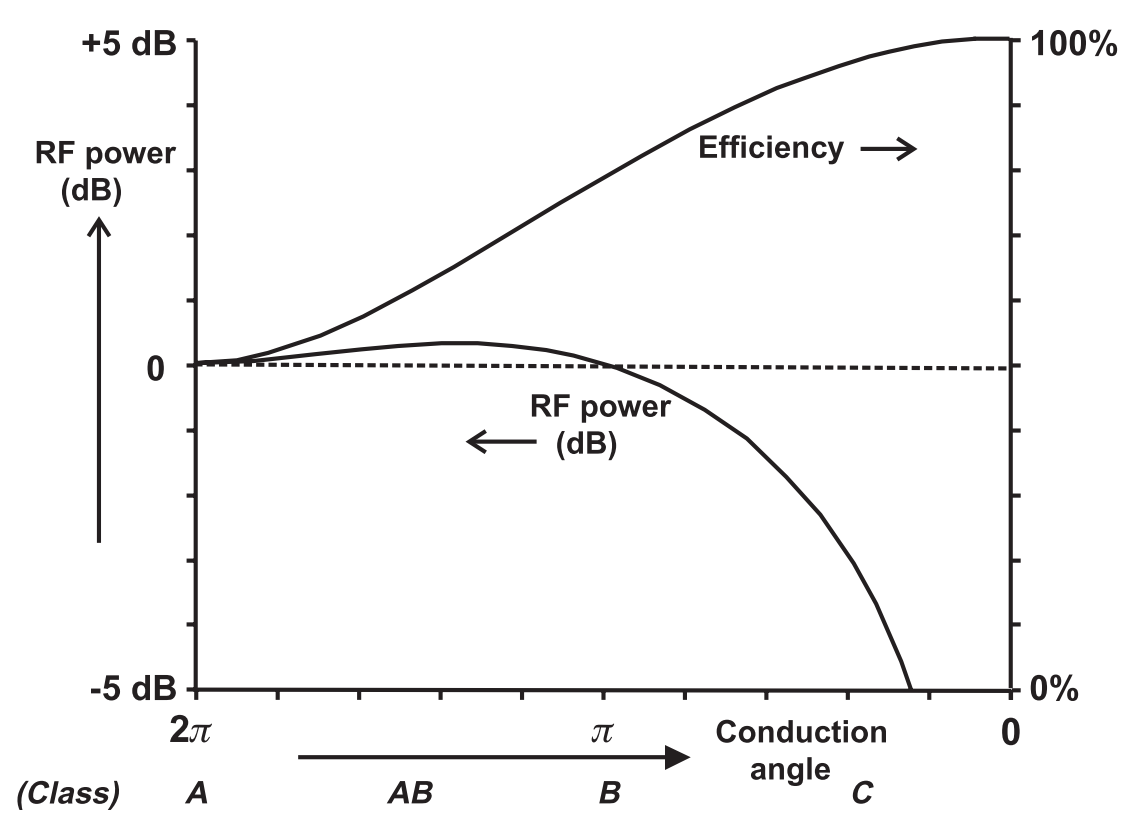
\includegraphics[width=4in,height=4in,keepaspectratio]{figures/classes/bias_power_eff}\\
  \caption{RF Power (relative to Class A) and Efficiency versus Conduction Angle \cite{C.Cripps2006}}
  \label{fig:bias_power_eff}
\end{figure}

\section{Switching Amplifiers}

Switching amplifiers model the transistor as a switch instead a dependent current source. Figure \ref{fig:basic_switch} shows the ideal operation of a switching amplifier. The transistor is modeled as a switch that can only be "on" or "off" depending on the gate voltage. The switching operation allows for current to flow while the switch is on with 0 drain voltage, and for 0 current while the switch is off with a non-zero drain voltage. Ideally this would allow for ZVS and for ZVDS which could result in 100\% efficiency. The switching amplifier classes (D, E, and F) build upon this ideal model and are able to achieve higher efficiencies in practice than current source amplifiers by using matching networks to shape the waveforms at the drain and gate.

\begin{figure}
    \subfigure{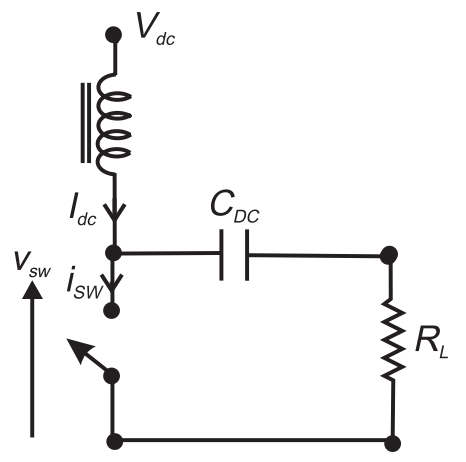
\includegraphics[width=3in]{figures/classes/basic_switch}}
    \subfigure{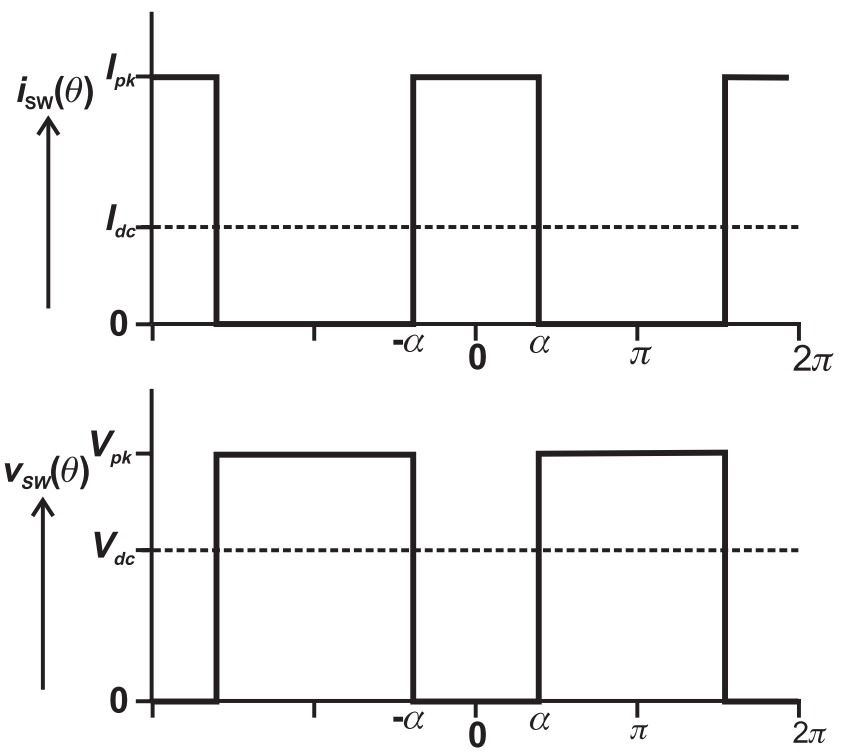
\includegraphics[width=3in]{figures/classes/basic_switch_waveform}}
    \caption{Basic Switching Amplifier Circuit and Waveforms\cite{C.Cripps2006}}\label{fig:basic_switch}
\end{figure}

\subsection{Class D Amplifier}

The class D amplifier can be thought of as push pull version of a switching amplifier. The amplifier consists of two transistors to operate as switches to conduct during the positive half and negative half cycle of the input seen in Figure \ref{fig:class_d} \cite{C.Cripps2006}. This allows for a full wave drain current to flow through the output load that is filtered through a high Q LC network while the drain voltage is a square wave with 0 overlap between the transistor that is on that allows for ZVS and ZVDS \cite{Rosu2001}. This allows the class D amplifier to theoretically have 100\% drain efficiency. The LC network is tuned to the fundamental frequency of the input. Class D looks effective in theory but suffers due to switching resistances and drain capacitances which limit the maximum frequency of operation to VHF in practice \cite{Raab2003}.

\begin{figure}
    \subfigure{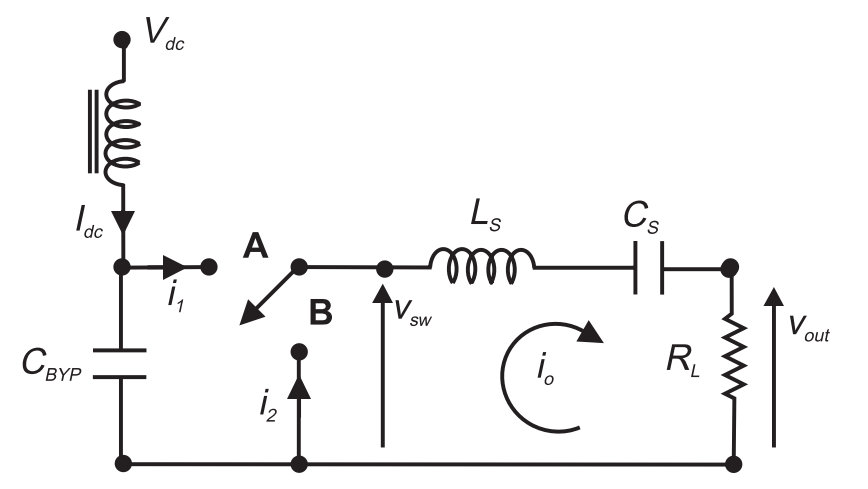
\includegraphics[width=3in]{figures/classes/classd_ckt}}
    \subfigure{{\raisebox{-0.25\height}{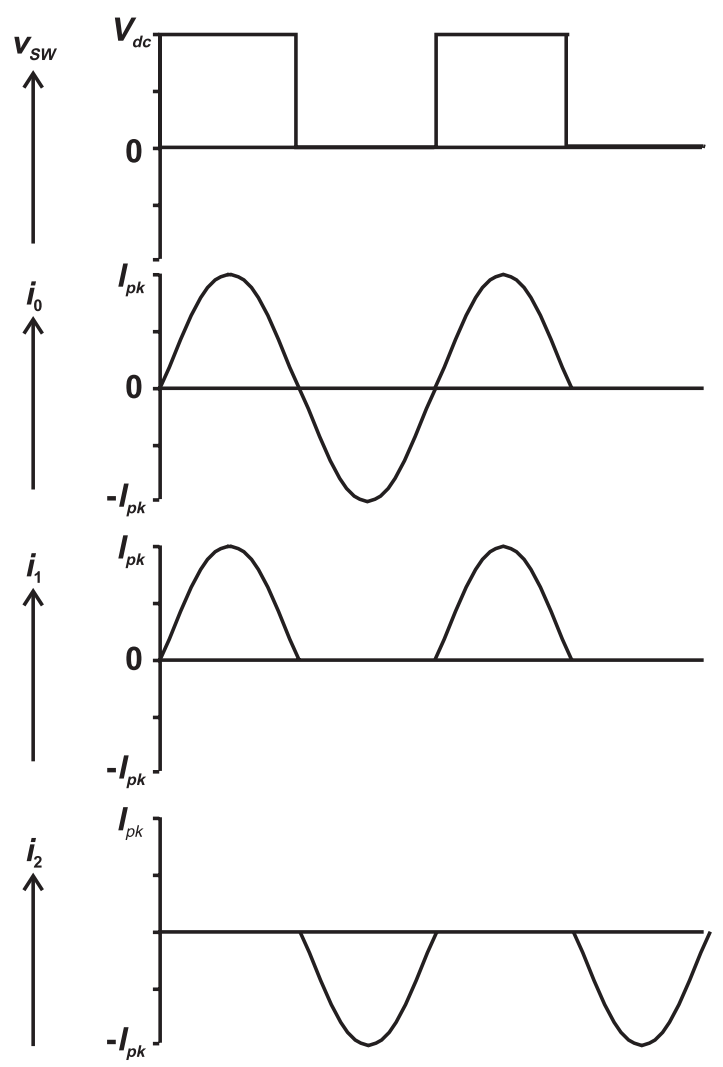
\includegraphics[width=3in,height=3in,keepaspectratio]{figures/classes/classd_wave}}}}
    \caption{Class D Amplifier Circuit and Waveforms\cite{C.Cripps2006}}\label{fig:class_d}
\end{figure}


\subsection{Class E Amplifier}

The class E amplifier builds up on the ideal switch amplifier takes in account for the shunt output drain capacitance and amplification is the result of DC and RF currents that charge the drain shunt capacitance \cite{Raab2003}. As seen in Figure \ref{fig:class_e}, the switch is turned on from  time $-\alpha_1$ to $\alpha_2$ allowing current to flow solely from the power supply and the load through the switch and the voltage across the drain capacitance is shorted. Then as the switch is turned off from time $\alpha_2$ to $\alpha_1$ the current from the power supply and load will flow through the drain capacitor \cite{C.Cripps2006}. To achieve high efficiency, the switching current waveforms are adjusted so that the capacitor current and charge is 0 when the switch is turned on which allows for ZVS and ZVDS conditions allowing for theoretically 100\% efficiency. \cite{Kee2003}.

The class E amplifier produces significant harmonic distortion due to the switching action and the output must be filtered to suppress harmonics \cite{Sokal1975}. Another concern with using the class E amplifier in practice is the large peak voltages at the drain of the transistor which are around three times the drain supply voltage when the switch turns off \cite{Hella}. In addition the output drain capacitance limits the frequency of operation that is required to create the proper drain waveforms \cite{Rosu2001}.

\begin{figure}
    \subfigure{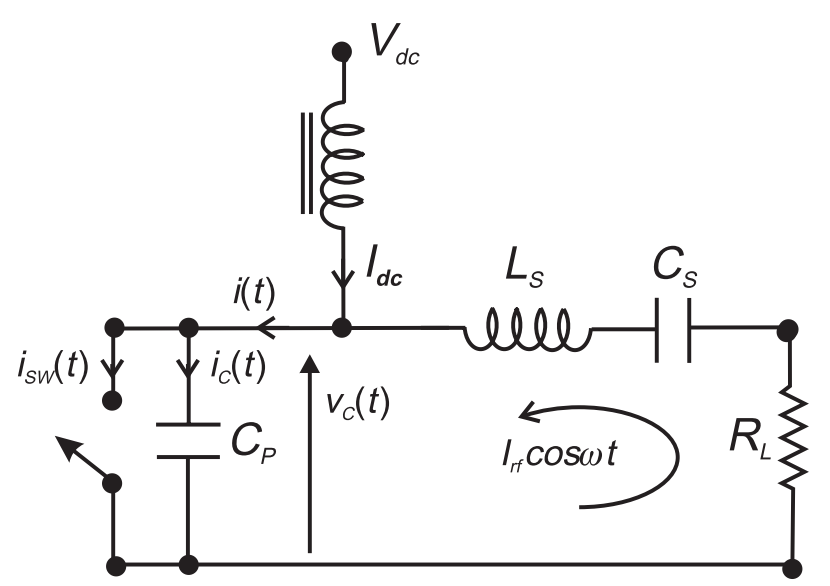
\includegraphics[width=3in]{figures/classes/classe_ckt}}
    \subfigure{{\raisebox{-0.25\height}{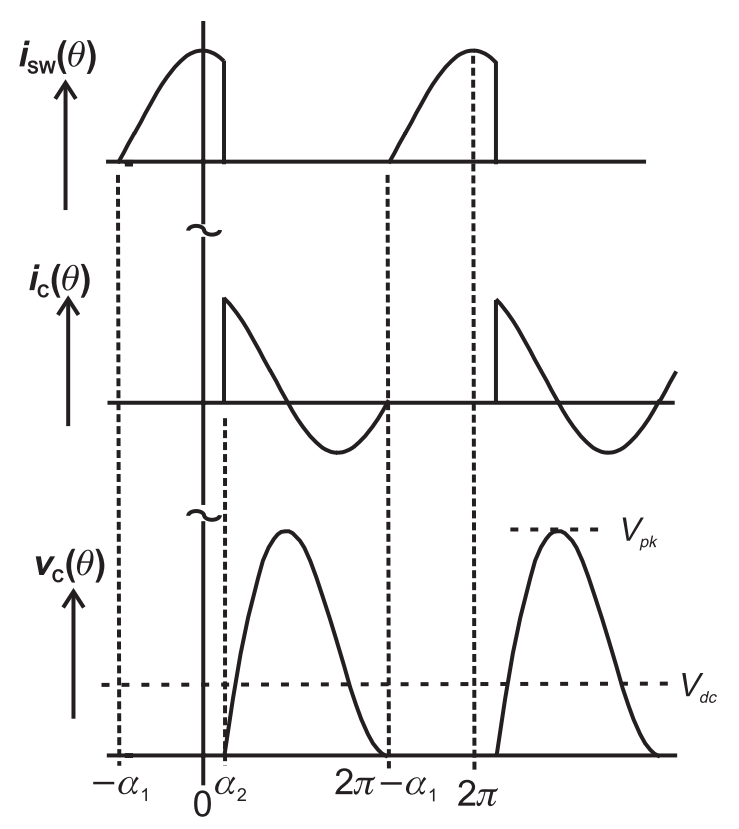
\includegraphics[width=3in,height=3in,keepaspectratio]{figures/classes/classe_wave2}}}}
    \caption{Class E Amplifier Circuit and Waveforms\cite{C.Cripps2006}}\label{fig:class_e}
\end{figure}

\subsection{Class F Amplifier}

The class F amplifier has a theoretical efficiency of 100\% through the use of multi harmonic terminations. The theory behind the class F amplifier relies on the generation of odd voltage harmonics and shorting of even voltage harmonics at the drain of the device to increase the efficiency of the amplifier. By keeping only the odd voltage harmonics of the signal at the output, ideally a square wave would appear and by biasing the amplifier at a conduction angle of pi the amplifier has zero overlap between the current and voltage waveforms and no power consumed when the amplifier is switched on.
The harmonics are generated due to the knee voltage of the transistor. When the AC signal causes the transistor to reach saturation the abrupt change in current flow generates voltage harmonics. In practice it becomes challenging to design matching networks as the number of harmonics to control increases. Also the output capacitance of the transistor will eventually short out higher order harmonics so 100\% efficiency is not realizable in practice. By controlling up to the 5th harmonic, 90.5\% efficiency can be achieved. A more in depth analysis of the class F amplifier follows in the next chapter.

%\subsection{Class J Amplifier}
%
%Shorts even harmonics
%
%Is described by the ratio of the drain reactance and the
%
%Maximum efficiency of 78.5\%

